\subsection{Benchmarks}
To evaluate how the hardware modifications improve the performance of core composition; the same benchmarks used in Chapter~\ref{chp:cases} are used here.
These benchmarks are all from the San-Diego Vision Benchmark Suite (SD-VBS)~\cite{sdvbs}, which is composed of a set of vision and image analysis applications, and are described in detail in Chapter~\ref{chp:setup} Section~\ref{chp:setup:sdvbs}.
The previous chapter showed that even with code optimisations, core compositions do not perform optimally when executing the benchmarks.
Some of the programs, such as \bm{MSER} or \bm{Multi\_NCut} features an average block size of under 10 instructions per block, making it difficult to use core composition efficiently.
They are therefore a perfect candidate to explore how the hardware modifications can improve the performance of core composition.

\begin{table}[t]
  \small
  \centering
 \begin{tabular} {| l | l | l | l | l | l | }
 \hline
   & \cellcolor[gray]{0.7}Disparity & \cellcolor[gray]{0.7} Localization& \cellcolor[gray]{0.7} MSER& \cellcolor[gray]{0.7} Multi\_NCut& \cellcolor[gray]{0.7} Sift\\ \hline
Input&	VGA  & VGA & CIF  & SIM\_FAST& CIF\\ \hline
	
	 & \cellcolor[gray]{0.7} Stitch & \cellcolor[gray]{0.7} SVM & \cellcolor[gray]{0.7} Text. Synth & \cellcolor[gray]{0.7} Tracking&\\ \hline
	  Input & CIF& CIF& FULLHD& VGA &\\ \hline

	\end{tabular}
  \caption{Datasets used for each of the benchmarks.}\label{tab:sd-data2}
\end{table}
\subsection{Evaluation} 
The previous chapter showed that the SD-VBS benchmarks feature repeating phases of IPC.
These benchmarks are structured as pipelines with distinct passes that are often times repeated.
This means that performance improvements can be analysed without having to fully execute the program.

As this chapter is only concerned with demonstrating that the new hardware modifications outperform the current implementation, the benchmarks are executed long enough to capture all the phases.
The phase data gathered from Chapter~\ref{chp:cases} is used to determine hotspots.
The benchmarks are then instrumented so that the main phases are captured, and executed for at least 100 million instructions.
Of that 100 million instructions, 10 million instructions are for warming up the caches and predictor.
Finally, the same data-sets from Chapter~\ref{chp:cases} are used, to maintain a consistency amongst the thesis; they can be found in Table~\ref{tab:sd-data2}.

\subsection{Value Predictor}

Value predictors that generate predictions both quickly and accurately are still actively being researched~\cite{peraisVTAGE2014,peraisBeBop2015,sheikh2017value}.
In order to motivate the use of value prediction for core composition, it is first important to abstract away current implementation details of state of the art predictors.
By considering a 100\% accurate prediction rate and immediate value prediction, this helps to determine how much value prediction can help improve performance.
Once the maximum speedup is determined, using a current state-of-the art implementation can help understand how far current value predictors are from the best performance.

This chapter explores two value predictors: a perfect value predictor that can predict any value in a single cycle, and a block based D-VTAGE~\cite{peraisBeBop2015} value predictor.
To have a better picture of how state-of-the art affects performance, different parameters of the predictor are modified.
This is discussed in further details in Section~\ref{chp:chp3:sec:analysis2}.

\subsection{Implementing perfect value and branch predictor}

\begin{figure}[t]
    \centering
    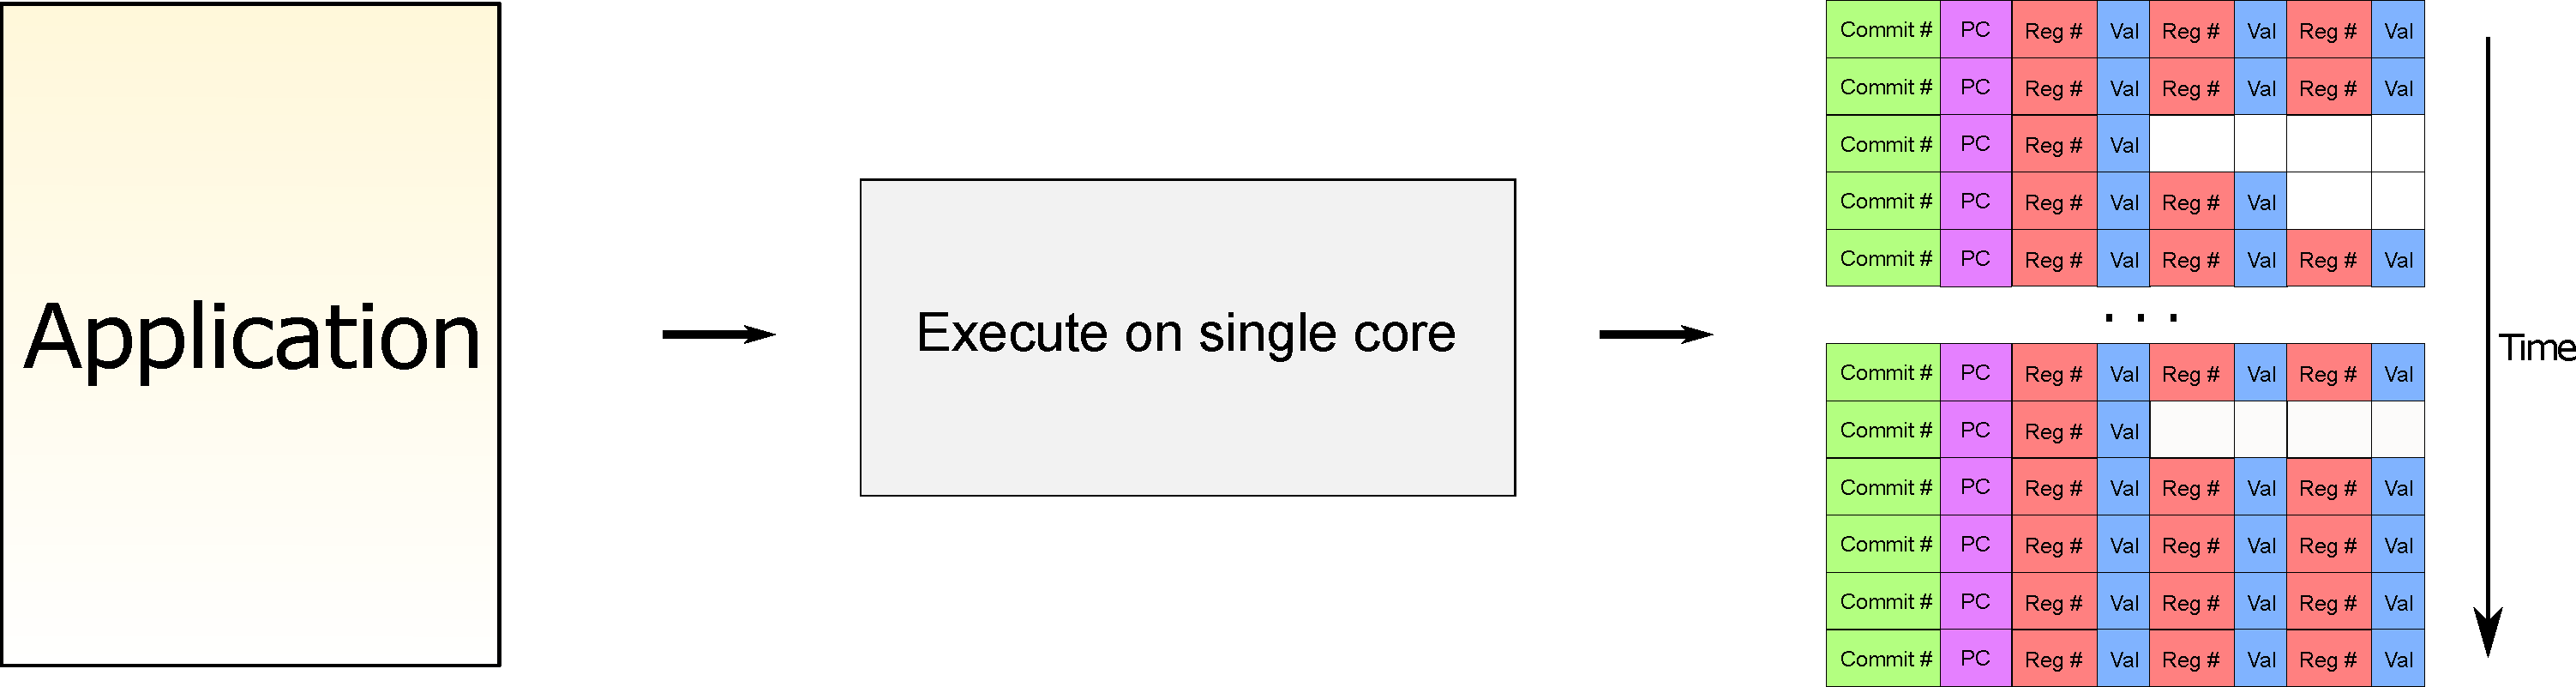
\includegraphics[width=1\textwidth]{chapter3/graphics/trace-gen.pdf}

    \caption{Overview of information gathering for generating traces which are used for the perfect branch and value predictors.}
    \label{fig:trace-gen}
\end{figure}

\begin{figure}[t]
    \centering
    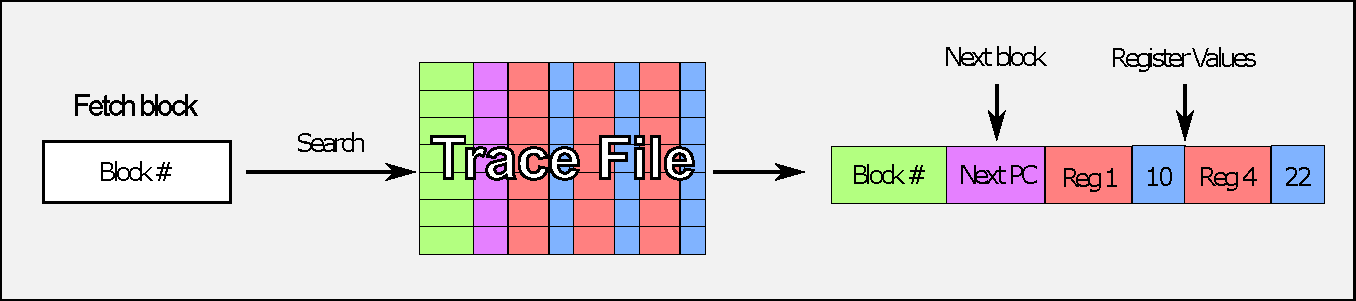
\includegraphics[width=1\textwidth]{chapter3/graphics/fetching-trace.pdf}

    \caption{Overview of how the trace data generated for value prediction is used during execution of a block.}
    \label{fig:trace-used}
	\vspace{1em}
\end{figure}

This chapter is concerned with how changing the hardware will improve the performance of core composition.
In order to motivate new research in branch prediction and value predictors and their use for core composition, it is essential to know what the maximum performance improvements are when using these techniques. %they're not techniques but you get the idea.
Thus, a perfect value predictor and branch predictor are considered for the analysis.

These predictors use execution traces of each application to make their predictions.
Figure~\ref{fig:trace-gen} shows how these traces are genereated.
The trace file contains an entry for every committed block, which is comprised of the Program Counter (PC) for the next block a list of registers that were read and their corresponding values.

When the perfect predictors are activated, the simulator reads in the trace file.
Figrue~\ref{fig:trace-used} shows how the trace data is used: a newly fetched block is paired with its correspondant trace data.
Instead of using the branch predictor, the next block's PC is directly taken from the trace entry, and whenever the block can issue a register read, the value is fetched from the trace entry instead of making a request to the register file.
\vspace{-2em}